\section{CNN accelerator overclocking} \label{sec:framework}
Overclocking can boot the clock frequency of CNN accelerators and is potentially beneficial to both 
the performance and energy efficiency. However, the timing violation may lead to distinct errors which 
may degrade the neural network prediction accuracy or even affect the functionality of the accelerators. 
To apply overclocking on CNN accelerators, we must handle all the possible 
problems incurred by the timing violation. 

\subsection{Overclocking overview}
Based on the intensity of overclocking and timing 
violation, we divide the overclocking incurred errors into different 
categories so that corresponding design methods can be used to 
alleviate the resulting problems efficiently. While it is difficult 
to precisely quantize the timing violation directly at runtime, we use 
the neural network prediction accuracy loss as the main 
classification metric. When there is only minor prediction accuracy 
loss which is less than 1\%, the penalty is usually acceptable 
and nothing needs to be done. When the prediction accuracy loss 
ranges from 1\% to 10\%, the moderate accuracy loss must be 
alleviated. When there is sever timing violation and 
accuracy loss, there is usually little chance to recover 
without improving the timing and the status of the accelerator 
may not be steady. It may result in considerable computing errors 
or even system stall due to critical control signal faults.  

As the critical paths may change at runtime due to the external 
environment variations such as temperature, the accuracy loss status may 
change as well. Typically, we expect that the lower overclocking setup 
may also lead to severe computing errors with relatively lower probability.
Fig \ref{fig:dynamic-loss} shows the possible accuracy loss status 
transition graph. It indicates that we should take the worst case 
into consideration even when the overclocking setup is relatively conservative.
\begin{figure}
	\center{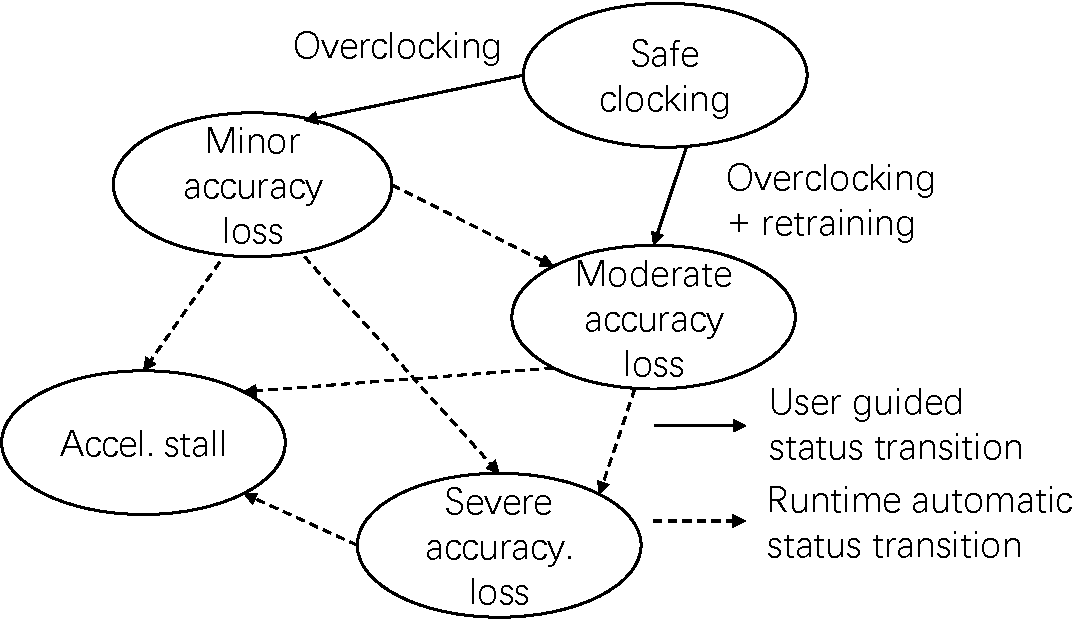
\includegraphics[width=0.75\linewidth]{overview}}
    \caption{CNN accelerator status transition graph.}
\label{fig:loss-estimation}
\vspace{-1em}
\end{figure}

For the minor accuracy loss case, overclocking can be used directly. 
We will not dwell on it. For the moderate accuracy loss, the neural network 
can still be salvaged. As the neural network models are usually obtained 
from offline training on general purposed processors (GPPs) which assumes the 
neural networks to be executed on an equivalent computing device, 
the computing on overclocked CNN accelerator varies and does not match 
with the assumption. To address this problem, we have the neural network models 
retrained on the overclocked accelerator so that the computing variation can be 
tolerated by the retrained models. By getting rid of the computing difference between 
inference and training, the prediction accuracy can be improved.

For the severe accuracy loss situation, the design can be hardly salvaged 
due to the relatively large amount of timing violations. In this case, 
we take advantage of the FPGA reconfiguration 
capability to reload an implementation with lower clock frequency. 
In some extreme case, the accelerator may even hang up. This can also be 
resolved with FPGA reconfiguration. However, the challenge is to 
detect the situation timely and recover the system automatically.

In combination with the possible accelerator status transfer graph and 
the related optimization approach, we propose an runtime overclocking 
management mechanism that ensures both efficient and resilient 
neural network computing. The mechanism is shown in Fig \ref{fig:runtime-management}.
\begin{figure}
	\center{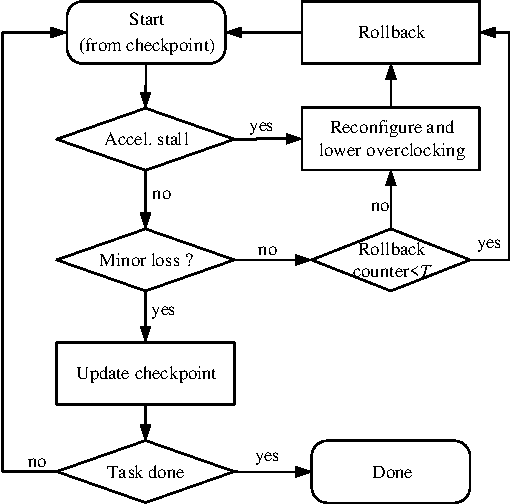
\includegraphics[width=0.45\linewidth]{manegment}}
    \caption{Runtime overclocking management.}
\label{fig:runtime-management}
\vspace{-1em}
\end{figure}

\subsection{Techniques for mitigating overclocking errors}
On top of the runtime overclocking management, we still need a series of techniques 
as mentioned in the above section to ensure resilient neural network processing 
on overclocked CNN accelerators. They will be detailed in this section.

\subsubsection{Accuracy loss estimation}
As illustrated in this section, typically a user may choose either the overclocking 
strategy with minor accuracy loss or moderate accuracy loss by setting up 
different clock frequency. Nevertheless, the critical paths 
may change at runtime with certain probability and the actual status of the CNN accelerator 
can be dynamic. Thus, it is of vital importance to detect the status of the CNN 
accelerator at runtime and activate the corresponding design strategy.

In order to determine the status of the overclocked CNN accelerators, 
we propose a runtime prediction accuracy loss estimation mechanism 
as shown in Fig \ref{fig:loss-estimation}. The basic idea is to insert a set 
of reference data to the input data stream. The actual prediction 
accuracy of the reference data can be computed in advance. When the 
reference data are processed on the overclocked CNN accelerator, the 
prediction accuracy of the refernce data can be obtained. By comparing the 
golden accuracy and the measured accuracy, we can calculate the accuracy loss and 
determine the status of the CNN accelerators accordingly. When the status of 
the accelerator is obtained, the corresponding optimization approach 
can be invoked. In addition, the amount of reference data inserted to 
the input data can be adjusted to ensure that the overhead is acceptable.

\begin{figure}
	\center{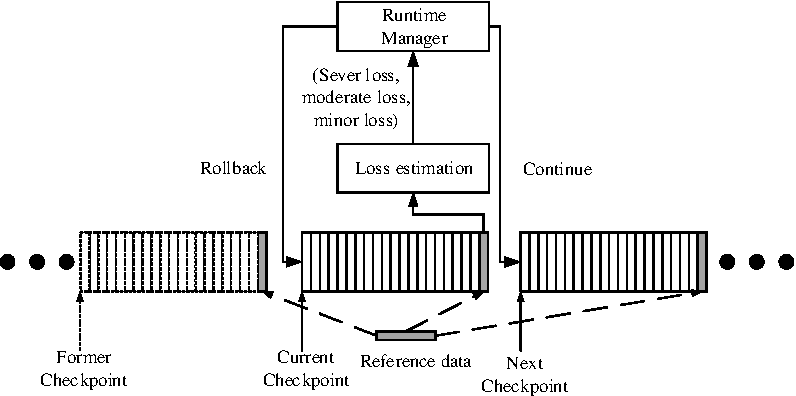
\includegraphics[width=0.85\linewidth]{loss_checkpoint}}
    \caption{Runtime neural network accuracy loss estimation.}
\label{fig:loss-estimation}
\vspace{-1em}
\end{figure}

On top of accuracy loss, the accelerator may hang up when the critical signals 
do not function as expected. Although a heart-beat mechansim may resolve this problem, 
it requires additional hardware design. To avoid introducing additional hardware, 
we use a simple timeout mechanism to determine whether the accelerator gets stuck. 

\subsubsection{On-accelerator retraining}
When there is moderate prediction accuracy loss due to the computing errors, 
we try to retrain the neural network model. The basic idea is to have both the 
applicaiton data and the computing variation patterns learned by the neural 
network model such that it can be less sensitive to the computing variations. 

Fig \ref{fig:retrain} shows the retraining framework built on top of Caffe.
The forward propagation that is usually performed on GPPs is transferred to 
the FPGA based CNN accelerator while the backward propagation remains the 
same. As the computing on the CNN accelerator is fixed point, the updated 
weight must be converted to fixed point before they are moved to FPGA 
for forward propagation. Accordingly, the result of the forward propagation 
needs to be converted to float point when it is sent to the host for backward 
propagation.

\begin{figure}
	\center{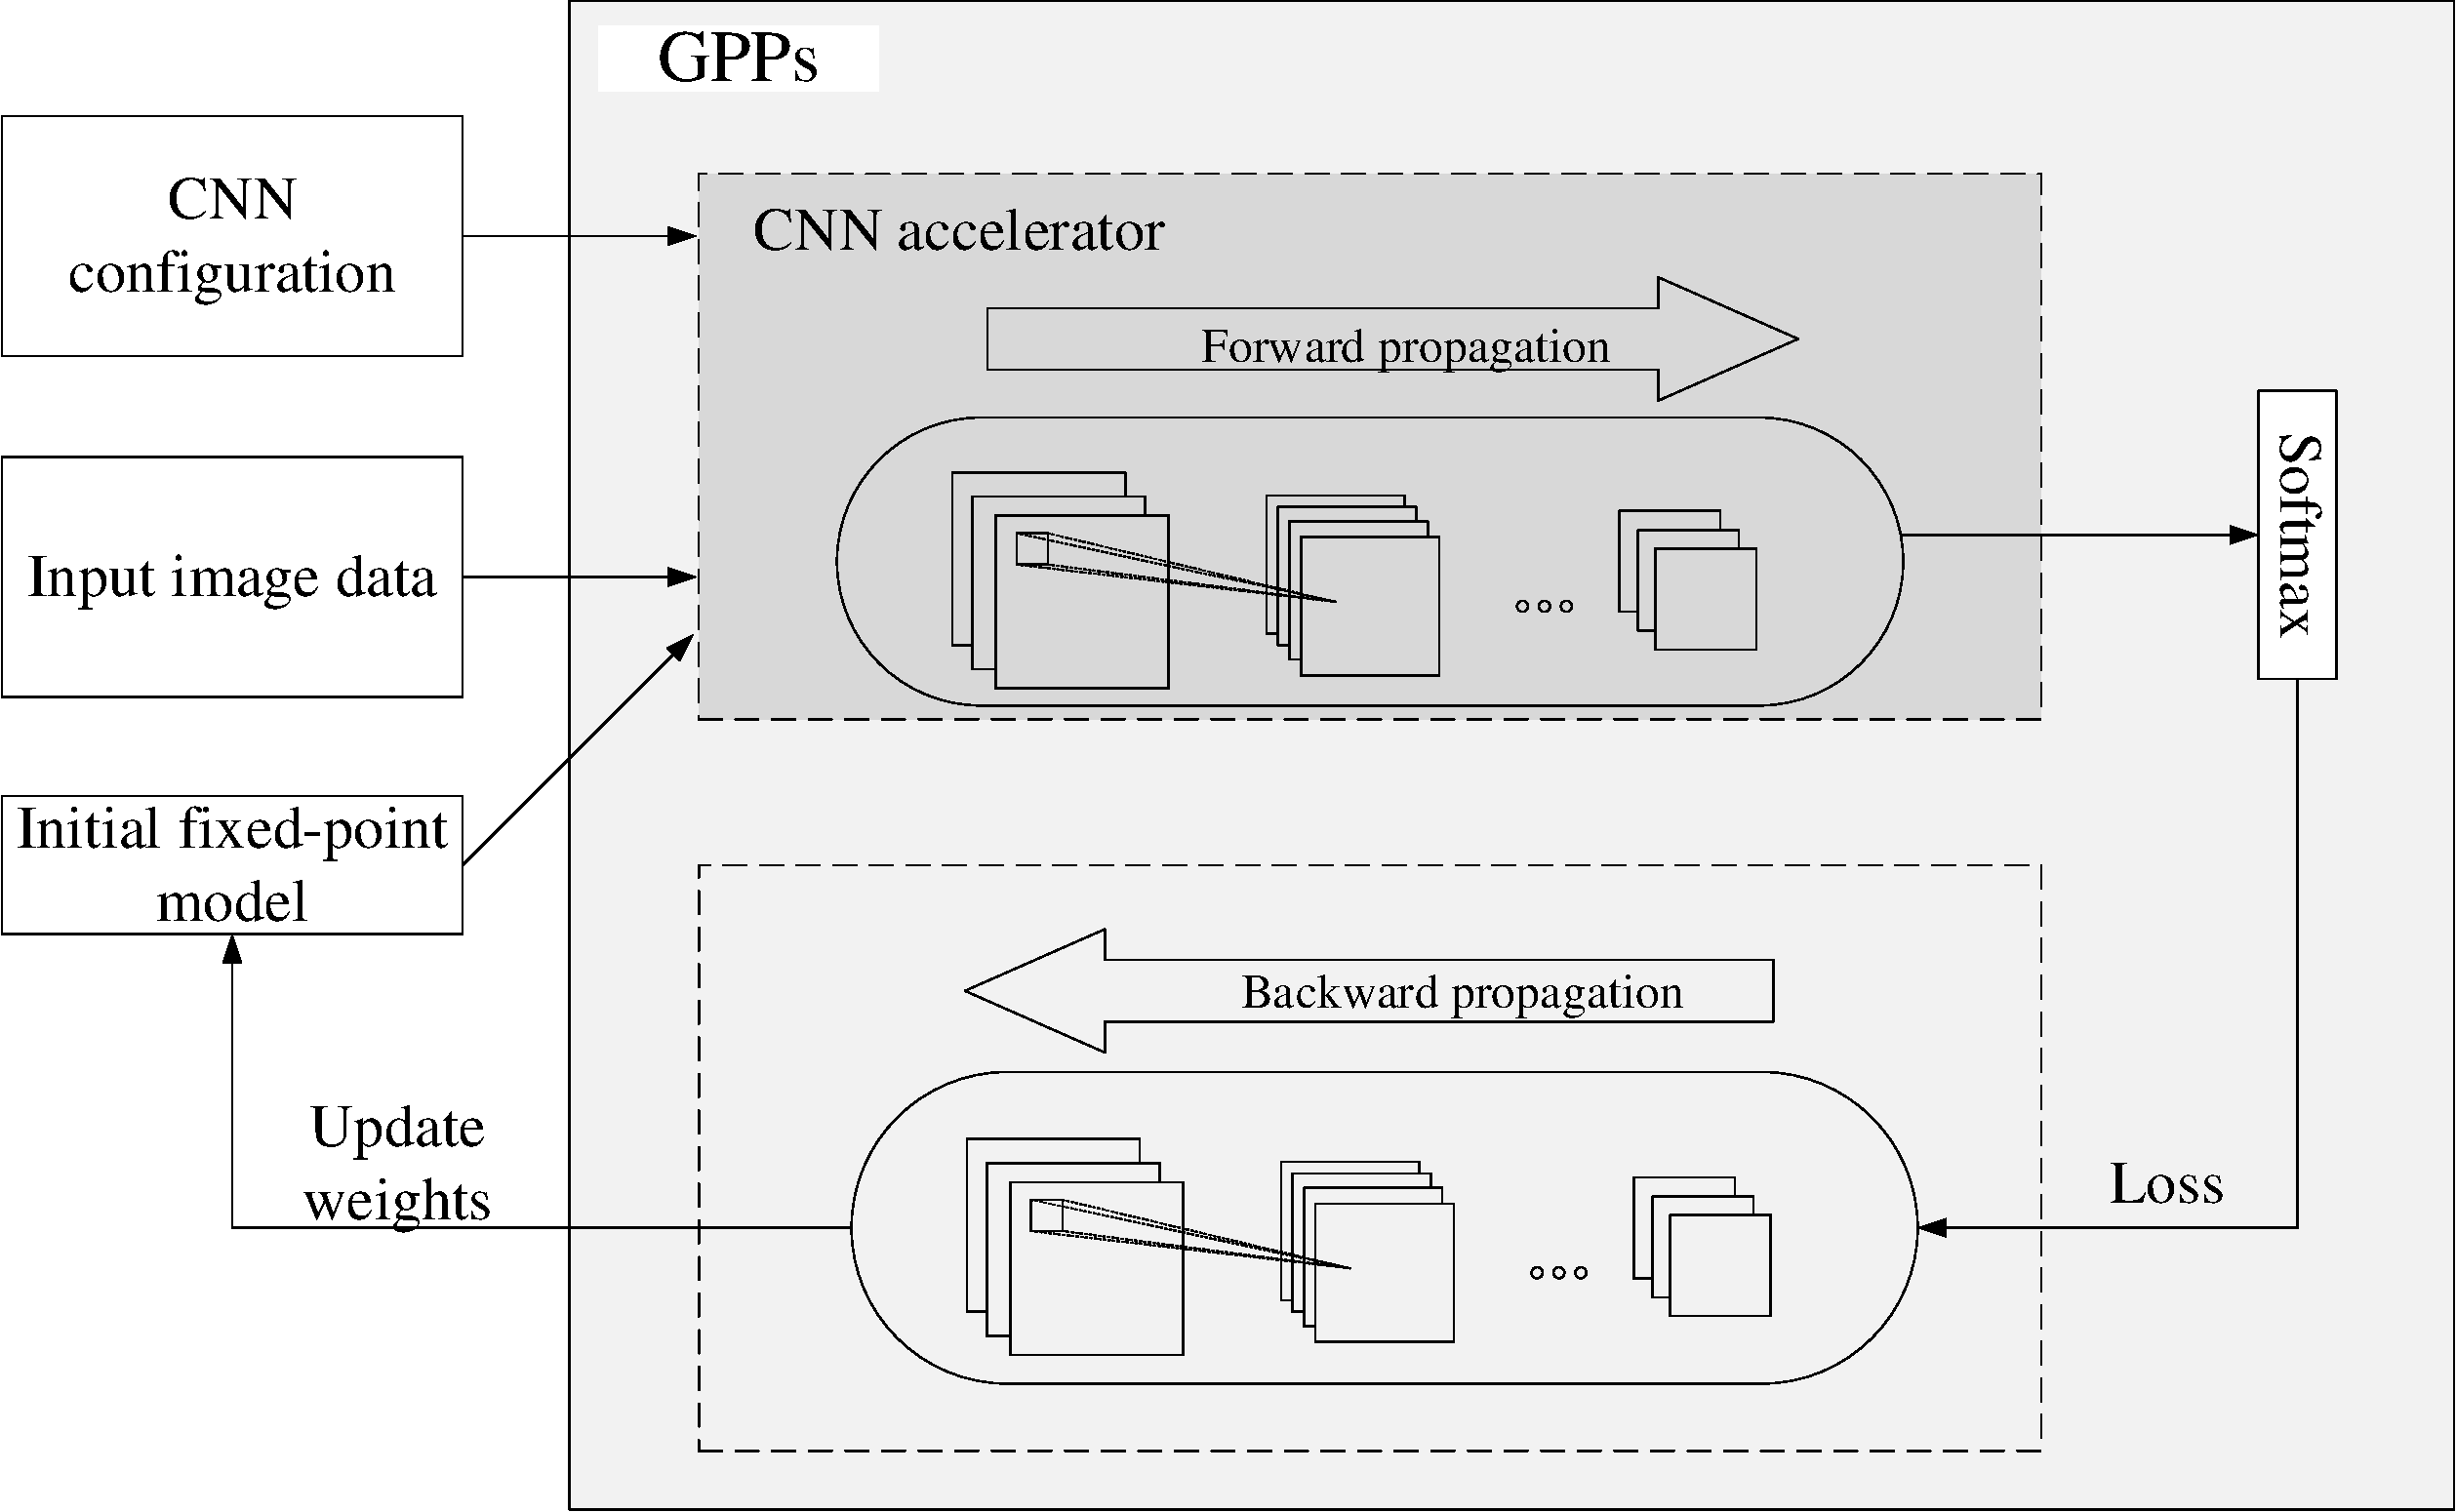
\includegraphics[width=0.85\linewidth]{retrain_framework}}
    \caption{On-accelerator neural network retraining framework.}
\label{fig:retrain}
\vspace{-1em}
\end{figure}


In this work, we utilized an OpenCL based CNN accelerator. The communication between 
host and the accelerator can be conveniently achieved with the OpenCL API. 
Nevertheless, many RTL based CNN accelerators can also be wrapped up with 
OpenCL API and reuse the retraining framework with minor modification.

\subsubsection{System reconfiguration and recovery}
When the accuracy loss gets too large, it indicates severe timing 
violations in the CNN accelerators which can be rather difficult to resolve with 
only fault-tolerant neural network models. Another extreme occasion is 
accelerator hangup when critical control signals are affected. In these cases, we 
opt to reconfigure the FPGA accelerator with a more conservative implementation.
However, when the errors are detected, previous computing may already suffer 
similar errors and many prediction can be wrong. To address this problem, we opt to 
utilize the checkpoint strategy to recover from previous checkpoint. 
Fig \ref{fig:checkpoint} shows the basic control flow of the checkpoint strategy.
Basically we divide the input data into blocks and some reference data 
will be added to the end of each block. When neural network accuracy measured with 
the reference data is abnormal, the processing will roll back to the last checkpoint 
which keeps the record of last input block index. Then we degrade the clock and 
new accelerator bitstream will be reloaded for the following inference.

%\begin{figure}
%	\center{
\includegraphics[width=0.75\linewidth]{blank}}
%    \caption{Checkpoint strategy for neural network computing fault recovery.}
%\label{fig:checkpoint}
%\vspace{-1em}
%\end{figure}


